We will now describe results obtained with \texttt{QuasinormalModes.jl}. We will not describe package usage since that topic is covered in details in the extensive package documentation, available online \href{https://lucass-carneiro.github.io/QuasinormalModes.jl/stable/}{here}. The code is hosted on GitHub and can be found in Ref.~\cite{QuasinormalModesRepo}. The package is registered in the \texttt{Julia} package index and can be easily installed with instructions provided in the \texttt{README} of the GitHub repository.

\subsection{Convergence and benchmarking}

We have written a \href{https://github.com/lucass-carneiro/QuasinormalModes.jl/tree/master/benchmark}{script} to test the package's performance and convergence characteristics. The script computes the fundamental $s=l=0$ mode of a Schwarzschild black hole while sweeping the number of AIM iterations from $n=1$ to $n=100$. The error of the computation as well as the time taken to compute the result and the number of iterations performed is repeated 20 times and each run is saved to a different text file in order to increase the statistical significance of the time measurements. The error measure is defined as the difference between AIM computed value and values obtained in Ref.~\cite{BertiQNMData} via Leaver's continued fraction method. The error convergence results are plotted in Figs.~\ref{fig:package_error} using a logarithmic scale in the $y$ axis for both the real (black dots) and imaginary (red crosses) parts of the mode a function the number of AIM iterations performed. It is possible to observe, despite oscillations, an overall trend of convergence towards the reference values. The (20 repetitions) average time taken as a function of the number of iterations is presented in Fig.~\ref{fig:package_perf} in a log-log plot. It is possible to see that the time taken increases with a power law trend as the number of AIM iterations gets higher.

\begin{figure}[!ht]
  \centering
  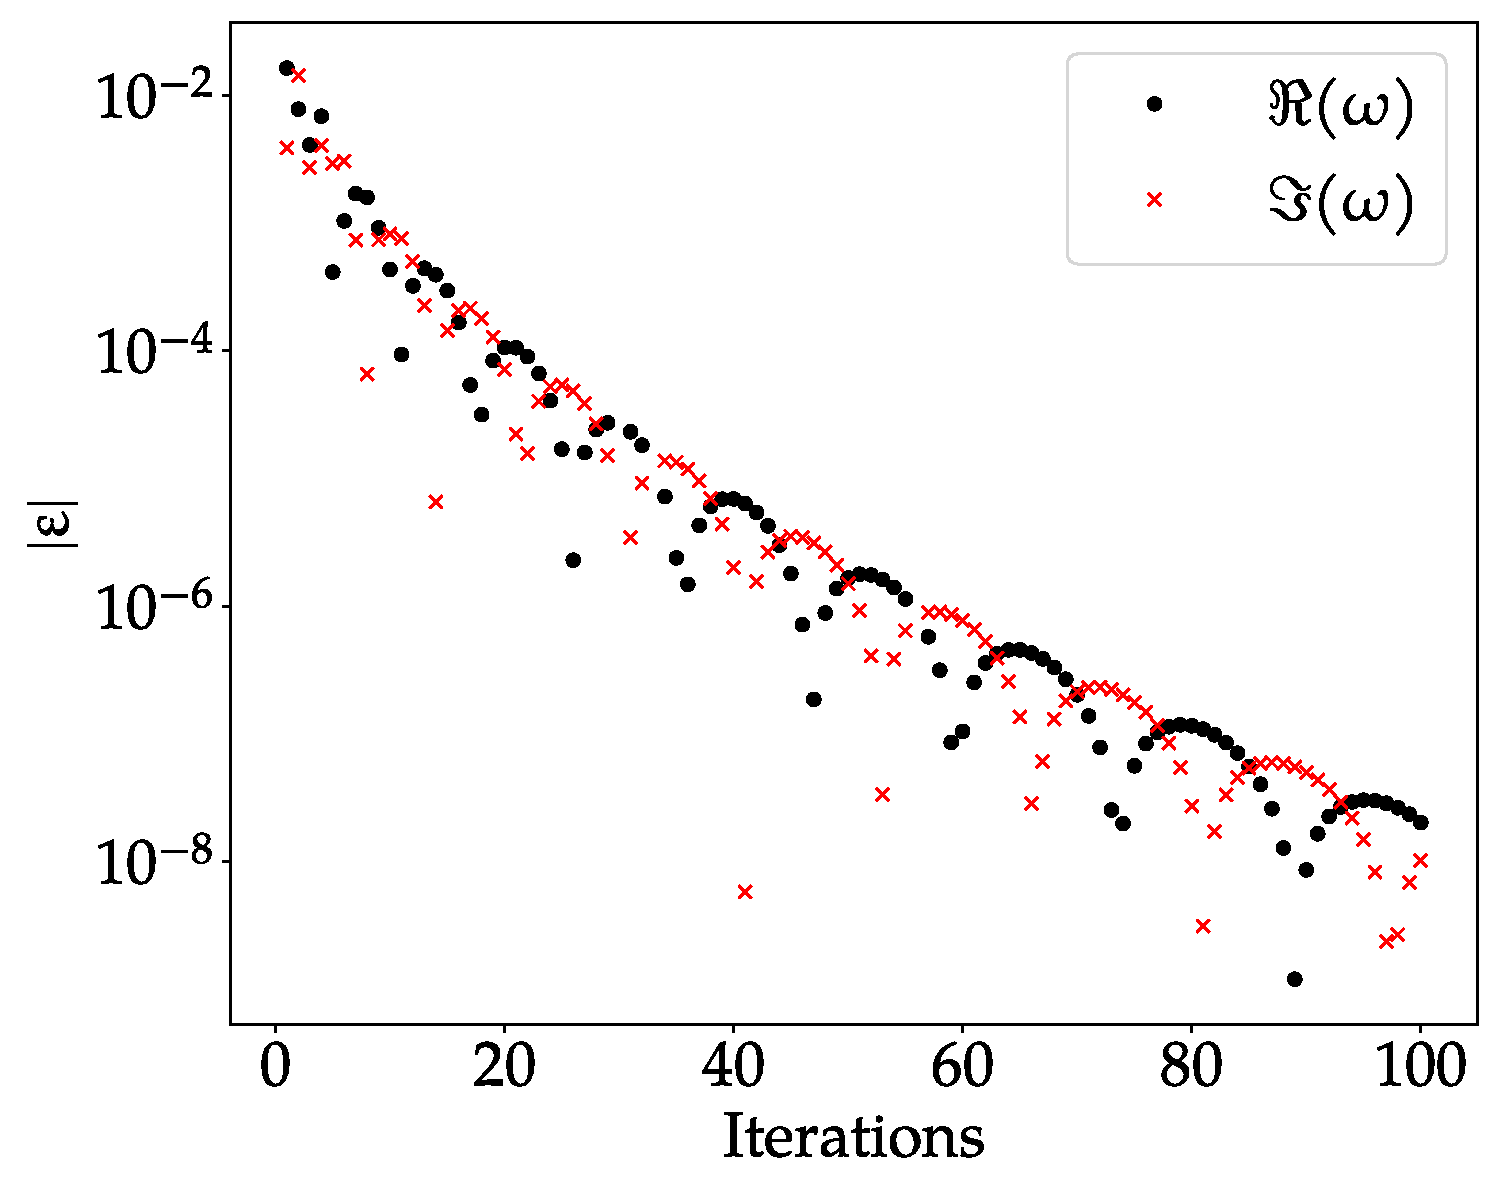
\includegraphics[scale = 0.35]{img/aim_qnm/err.pdf}
  \caption{Error of the fundamental $s=l=0$ Schwarzschild QNM vs. the number of AIM iterations. Reference values obtained in Ref.~\cite{BertiQNMData}. The y-axis of the plot is in logarithmic scale.}
  \label{fig:package_error}
\end{figure}

\begin{figure}[!ht]
  \centering
  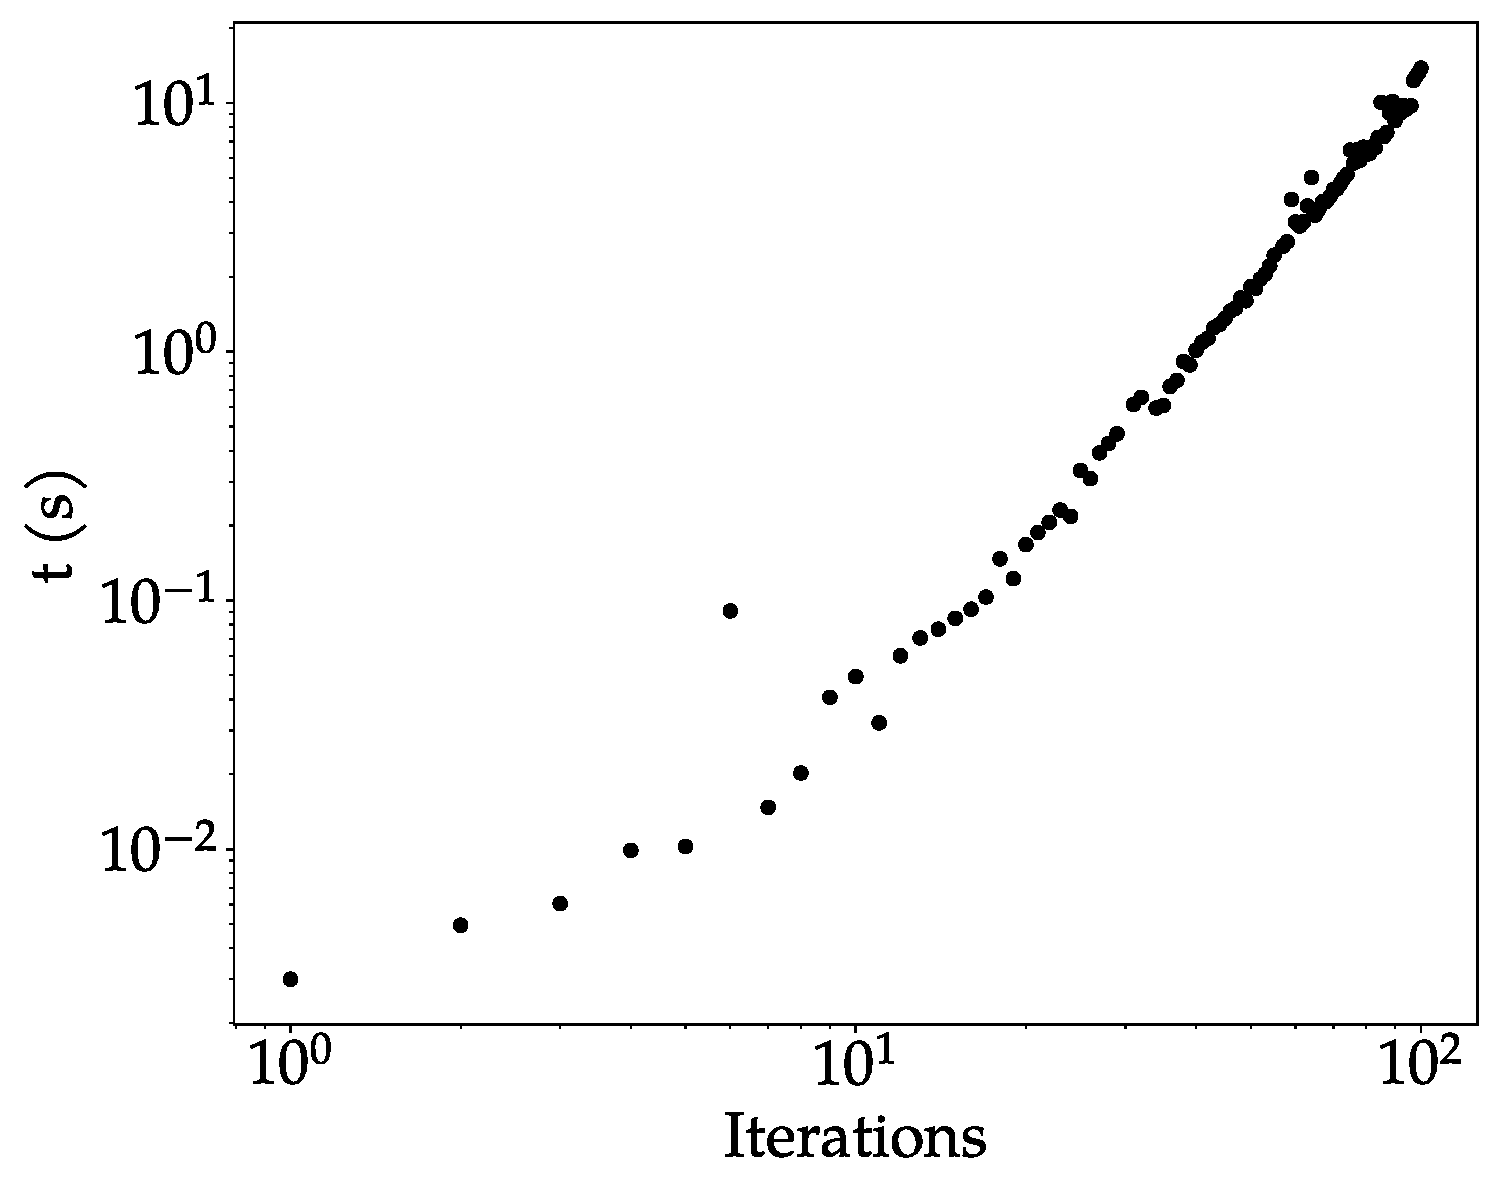
\includegraphics[scale = 0.35]{img/aim_qnm/perf.pdf}
  \caption{Time taken (average of 20 repetitions) vs. the number of AIM iterations taken to compute the fundamental Schwarzschild QNM. The plot is in a log-log scale.}
  \label{fig:package_perf}
\end{figure}

\subsection{Comparison with pseudo-spectral methods}

We have, with collaborators in Ref.~\cite{Mamani2022}, revisited the problem of computing QNMs resulting from perturbations of spins $0$, $1/2$, $1$, $3/2$, $2$, $5/2$ of an asymptotically flat Schwarzschild black hole. Our aim was to compare numerical results obtained via the AIM with those obtained using the pseudo-spectral method and contrast both results with data available in the literature whenever possible. We have computed higher overtones quasinormal frequencies for all the investigated perturbation fields and obtained  purely imaginary frequencies for spin $1/2$ and $3/2$ fields that are in agreement with analytic results reported previously in the literature. The purely imaginary frequencies for the spin $1/2$ perturbation field are exactly the same as the frequencies obtained for the spin $3/2$ perturbation field. Finally, we computed, the quasinormal frequencies for the spin $5/2$ perturbation field for the very first time, and purely imaginary frequencies are found also in this case.

\subsubsection{Integer spin results}


\begin{table}[ht]
  \centering
  \scalebox{0.62}{
    \begin{tabular}{l |c|c|c|c|c|c}
      \hline
      $l$ & $n$ & \tlt{Pseudo-spectral}{I (60 Polynomials)} & \tlt{Pseudo-spectral}{II (40 polynomials)} & \tlt{AIM}{100 Iterations}  & Ref.~\cite{Shu:2005fw} & Ref.~\cite{Konoplya:2004ip} \\ \hline\hline
      0   & $0$ & $\pm 0.110455 -0.104896 i$                & $\pm 0.110455 -0.104896 i$                 & $\pm 0.110455 -0.104896 i$ & $0.1046-0.1152 i$      & $\pm 0.1105-0.1008i$        \\ \hline
      1   & $0$ & $\pm 0.292936 -0.097660 i$                & $\pm 0.292936 -0.097660 i$                 & $\pm 0.292936 -0.097660 i$ & $0.2911-0.0980 i$      & $\pm 0.2929-0.0978i$        \\
          & $1$ & $\pm 0.264449 -0.306257 i$                & $\pm 0.264449 -0.306257 i$                 & $\pm 0.264449 -0.306257 i$ & ---                    & $\pm 0.2645-0.3065i$        \\ \hline
      2   & $0$ & $\pm 0.483644 -0.096759 i$                & $\pm 0.483644 -0.096759 i$                 & $\pm 0.483644 -0.096759 i$ & $0.4832-0.0968 i$      & $\pm 0.4836-0.0968i$        \\
          & $1$ & $\pm 0.463851 -0.295604 i$                & $\pm 0.463851 -0.295604 i$                 & $\pm 0.463851 -0.295604 i$ & $0.4632-0.2958 i$      & $\pm 0.4638-0.2956i$        \\
          & $2$ & $\pm 0.430544 -0.508558 i$                & $\pm 0.430544 -0.508558 i$                 & $\pm 0.430544 -0.508558 i$ & ---                    & $\pm 0.4304-0.5087i$        \\ \hline
      3   & $0$ & $\pm 0.675366 -0.096500 i$                & $\pm 0.675366 -0.096500 i$                 & $\pm 0.675366 -0.096500 i$ & $0.6752-0.0965 i$      & ---                         \\
          & $1$ & $\pm 0.660671 -0.292285 i$                & $\pm 0.660671 -0.292285 i$                 & $\pm 0.660671 -0.292285 i$ & $0.6604-0.2923 i$      & ---                         \\
          & $2$ & $\pm 0.633626 -0.496008 i$                & $\pm 0.633626 -0.496008 i$                 & $\pm 0.633626 -0.496008 i$ & $0.6348-0.4941 i$      & ---                         \\
          & $3$ & $\pm 0.598773 -0.711221 i$                & $\pm 0.598773 -0.711221 i$                 & $\pm 0.598773 -0.711221 i$ & ---                    & ---                         \\ \hline
      4   & $0$ & $\pm 0.867416 -0.096392 i$                & $\pm 0.867416 -0.096392 i$                 & $\pm 0.867416 -0.096392 i$ & $0.8673-0.0964 i$      & ---                         \\
          & $1$ & $\pm 0.855808 -0.290876 i$                & $\pm 0.855808 -0.290876 i$                 & $\pm 0.855808 -0.290876 i$ & $0.8557-0.2909 i$      & ---                         \\
          & $2$ & $\pm 0.833692 -0.490325 i$                & $\pm 0.833692 -0.490325 i$                 & $\pm 0.833692 -0.490325 i$ & $0.8345-0.4895 i$      & ---                         \\
          & $3$ & $\pm 0.803288 -0.697482 i$                & $\pm 0.803288 -0.697482 i$                 & $\pm 0.803288 -0.697482 i$ & $0.8064-0.6926 i$      & ---                         \\
          & $4$ & $\pm 0.767733 -0.914019 i$                & $\pm 0.767733 -0.914019 i$                 & $\pm 0.767733 -0.914019 i$ & ---                    & ---                         \\
      \hline\hline
    \end{tabular}
  }
  \caption{
    Quasinormal frequencies of the spin $0$ perturbations normalized by the mass $(M\omega)$ compared against the results of Refs.~\cite{Shu:2005fw, Konoplya:2004ip}.
  }
  \label{Tab:Spin0}
\end{table}

\begin{table}[ht]
  \centering
  \scalebox{0.62}{
    \begin{tabular}{l |c|c|c|c|c|c}
      \hline
      $l$ & $n$ & \tlt{Pseudo-spectral}{I (60 Polynomials)} & \tlt{Pseudo-spectral}{II (40 polynomials)} & \tlt{AIM}{100 Iterations}  & Ref.~\cite{Shu:2005fw} & Ref.~\cite{Konoplya:2004ip} \\ \hline\hline
      1   & $0$ & $\pm 0.248263-0.092488 i$                 & $\pm 0.248263 -0.092488 i$                 & $\pm 0.248263 -0.092488 i$ & $0.2459-0.0931i$       & $\pm 0.2482-0.0926i$        \\
          & $1$ & $\pm 0.214515-0.293668 i$                 & $\pm 0.214515 -0.293667 i$                 & $\pm 0.214515 -0.293668 i$ & ---                    & $\pm 0.2143-0.2941i$        \\ \hline
      2   & $0$ & $\pm 0.457596-0.095004 i$                 & $\pm 0.457595 -0.095004 i$                 & $\pm 0.457596 -0.095004 i$ & $0.4571-0.0951i$       & $\pm 0.4576-0.0950i$        \\
          & $1$ & $\pm 0.436542-0.290710 i$                 & $\pm 0.436542 -0.290710 i$                 & $\pm 0.436542 -0.290710 i$ & $0.4358-0.2910i$       & $\pm 0.4365-0.2907i$        \\
          & $2$ & $\pm 0.401187-0.501587 i$                 & $\pm 0.401187 -0.501587 i$                 & $\pm 0.401187 -0.501587 i$ & ---                    & $\pm 0.4009-0.5017i$        \\ \hline
      3   & $0$ & $\pm 0.656899-0.095616 i$                 & $\pm 0.656899 -0.095616 i$                 & $\pm 0.656899 -0.095616 i$ & $0.6567-0.0956i$       & $\pm 0.6569-0.0956i$        \\
          & $1$ & $\pm 0.641737-0.289728 i$                 & $\pm 0.641737 -0.289728 i$                 & $\pm 0.641737 -0.289728 i$ & $0.6415-0.2898i$       & $\pm 0.6417-0.2897i$        \\
          & $2$ & $\pm 0.613832-0.492066 i$                 & $\pm 0.613832 -0.492066 i$                 & $\pm 0.613832 -0.492066 i$ & $0.6151-0.4901i$       & $\pm 0.6138-0.4921i$        \\
          & $3$ & $\pm 0.577919-0.706331 i$                 & $\pm 0.577919 -0.706331 i$                 & $\pm 0.577919 -0.706330 i$ & ---                    & $\pm 0.5775-0.7065i$        \\ \hline
      4   & $0$ & $\pm 0.853095-0.095860 i$                 & $\pm 0.853095 -0.095860 i$                 & $\pm 0.853095 -0.095810 i$ & $0.8530-0.0959i$       & ---                         \\
          & $1$ & $\pm 0.841267-0.289315 i$                 & $\pm 0.841267 -0.289315 i$                 & $\pm 0.841267 -0.289315 i$ & $0.8411-0.2893i$       & ---                         \\
          & $2$ & $\pm 0.818728-0.487838 i$                 & $\pm 0.818728 -0.487838 i$                 & $\pm 0.818728 -0.487838 i$ & $0.8196-0.4870i$       & ---                         \\
          & $3$ & $\pm 0.787748-0.694242 i$                 & $\pm 0.787748 -0.694242 i$                 & $\pm 0.787748 -0.694242 i$ & $0.7909-0.6892i$       & ---                         \\
          & $4$ & $\pm 0.751549-0.910242 i$                 & $\pm 0.751549 -0.910242 i$                 & $\pm 0.751549 -0.910242 i$ & ---                    & ---                         \\
      \hline\hline
    \end{tabular}
  }
  \caption{
    Quasinormal frequencies of the spin $1$ perturbations normalized by the mass $(M\omega)$ compared against the results of Refs.~\cite{Shu:2005fw, Konoplya:2004ip}.
  }
  \label{Tab:Spin1}
\end{table}

\begin{table}[ht]
  \centering
  \scalebox{0.62}{
    \begin{tabular}{l |c|c|c|c|c|c}
      \hline
      $l$ & $n$ & \tlt{Pseudo-spectral}{I (60 Polynomials)} & \tlt{Pseudo-spectral}{II (40 polynomials)} & \tlt{AIM}{100 Iterations}  & Ref.~\cite{Shu:2005fw} & Ref.~\cite{Konoplya:2004ip} \\ \hline\hline
      2   & $0$ & $\pm 0.373672-0.088962i$                  & $\pm 0.373672 -0.088962 i$                 & $\pm 0.373672 -0.088962 i$ & $0.3730-0.0891i$       & $\pm 0.3736-0.0890i$        \\
          & $1$ & $\pm 0.346711-0.273915i$                  & $\pm 0.346711 -0.273915 i$                 & $\pm 0.346711 -0.273915 i$ & $0.3452-0.2746i$       & $\pm 0.3463-0.2735i$        \\
          & $2$ & $\pm 0.301053-0.478277i$                  & $\pm 0.301053 -0.478277 i$                 & $\pm 0.301053 -0.478277 i$ & ---                    & $\pm 0.2985-0.4776i$        \\ \hline
      3   & $0$ & $\pm 0.599443-0.092703i$                  & $\pm 0.599443 -0.092703 i$                 & $\pm 0.599443 -0.092703 i$ & $0.5993-0.0927i$       & $\pm 0.5994-0.0927i$        \\
          & $1$ & $\pm 0.582644-0.281298i$                  & $\pm 0.582644 -0.281298 i$                 & $\pm 0.582644 -0.281298 i$ & $0.5824-0.2814i$       & $\pm 0.5826-0.2813i$        \\
          & $2$ & $\pm 0.551685-0.479093i$                  & $\pm 0.551685 -0.479093 i$                 & $\pm 0.551685 -0.479027 i$ & $0.5532-0.4767i$       & $\pm 0.5516-0.4790i$        \\
          & $3$ & $\pm 0.511962-0.690337i$                  & $\pm 0.511962 -0.690337 i$                 & $\pm 0.511962 -0.690337 i$ & ---                    & $\pm 0.5111-0.6905i$        \\ \hline
      4   & $0$ & $\pm 0.809178-0.094164i$                  & $\pm 0.809178 -0.094164 i$                 & $\pm 0.809178 -0.094164 i$ & $0.8091-0.0942i$       & $\pm 0.8092-0.0942i$        \\
          & $1$ & $\pm 0.796632-0.284334i$                  & $\pm 0.796632 -0.284334 i$                 & $\pm 0.796632 -0.284334 i$ & $0.7965-0.2844i$       & $\pm 0.7966-0.2843i$        \\
          & $2$ & $\pm 0.772710-0.479908i$                  & $\pm 0.772710 -0.479908 i$                 & $\pm 0.772710 -0.479908 i$ & $0.7736-0.4790i$       & $\pm 0.7727-0.4799i$        \\
          & $3$ & $\pm 0.739837-0.683924i$                  & $\pm 0.739837 -0.683924 i$                 & $\pm 0.739837 -0.683924 i$ & $0.7433-0.6783i$       & $\pm 0.7397-0.6839i$        \\
          & $4$ & $\pm 0.701516-0.898239i$                  & $\pm 0.701516 -0.898239 i$                 & $\pm 0.701516 -0.898239 i$ & ---                    & $\pm 0.7006-0.8985i$        \\
      \hline\hline
    \end{tabular}
  }
  \caption{
    Quasinormal frequencies of spin $2$ perturbations normalized by the mass $(M\omega)$ compared against the results of Refs.~\cite{Shu:2005fw, Konoplya:2004ip}.
  }
  \label{Tab:Spin2}
\end{table}

\subsubsection{Semi-integer spin}

\begin{table}[ht]
  \centering
  \scalebox{0.62}{
    \begin{tabular}{l |c|c|c|c|c|c}
      \hline
      $l$ & $n$ & \tlt{Pseudo-spectral}{I (60 Polynomials)} & \tlt{Pseudo-spectral}{II (40 polynomials)} & \tlt{AIM}{100 Iterations}  & Ref.~\cite{Shu:2005fw} & Ref.~\cite{Cho:2003qe} \\ \hline\hline
      0   & $0$ & $\pm 0.182963 -0.096982 i$                & $\pm 0.182963 -0.096982 i$                 & $\pm 0.182963 -0.096824 i$ & ---                    & ---                    \\ \hline
      1   & $0$ & $\pm 0.380037 -0.096405 i$                & $\pm 0.380037 -0.096405 i$                 & $\pm 0.380037 -0.096405 i$ & $0.3786-0.0965 i$      & $0.379 -0.097i$        \\
          & $1$ & $\pm 0.355833 -0.297497 i$                & $\pm 0.355833 -0.297497 i$                 & $\pm 0.355833 -0.297497 i$ & ---                    & ---                    \\ \hline
      2   & $0$ & $\pm 0.574094 -0.096305 i$                & $\pm 0.574094 -0.096305 i$                 & $\pm 0.574094 -0.096305 i$ & $0.5737-0.0963 i$      & $0.574 -0.096i$        \\
          & $1$ & $\pm 0.557015 -0.292715 i$                & $\pm 0.557015 -0.292715 i$                 & $\pm 0.557015 -0.292715 i$ & $0.5562-0.2930 i$      & $0.556 -0.293i$        \\
          & $2$ & $\pm 0.526607 -0.499695 i$                & $\pm 0.526607 -0.499695 i$                 & $\pm 0.526607 -0.499695 i$ & ---                    & ---                    \\ \hline
      3   & $0$ & $\pm 0.767355 -0.096270 i$                & $\pm 0.767355 -0.096270 i$                 & $\pm 0.767355 -0.096270 i$ & $0.7672-0.0963 i$      & $0.767 -0.096i$        \\
          & $1$ & $\pm 0.754300 -0.290968 i$                & $\pm 0.754300 -0.290968 i$                 & $\pm 0.754300 -0.290968 i$ & $0.7540-0.2910 i$      & $0.754 -0.291i$        \\
          & $2$ & $\pm 0.729770 -0.491910 i$                & $\pm 0.729770 -0.491910 i$                 & $\pm 0.729770 -0.491910 i$ & $0.7304-0.4909 i$      & $0.730 -0.491i$        \\
          & $3$ & $\pm 0.696913 -0.702293 i$                & $\pm 0.696913 -0.702293 i$                 & $\pm 0.696913 -0.702293 i$ & ---                    & ---                    \\ \hline
      4   & $0$ & $\pm 0.960293 -0.096254 i$                & $\pm 0.960293 -0.096254 i$                 & $\pm 0.960293 -0.096254 i$ & $0.9602-0.0963 i$      & $0.960 -0.096i$        \\
          & $1$ & $\pm 0.949759 -0.290148 i$                & $\pm 0.949759 -0.290148 i$                 & $\pm 0.949759 -0.290148 i$ & $0.9496-0.2902 i$      & $0.950 -0.290i$        \\
          & $2$ & $\pm 0.929494 -0.488116 i$                & $\pm 0.929494 -0.488116 i$                 & $\pm 0.929494 -0.488116 i$ & $0.9300-0.4876 i$      & $0.930 -0.488i$        \\
          & $3$ & $\pm 0.901129 -0.692520 i$                & $\pm 0.901129 -0.692520 i$                 & $\pm 0.901129 -0.692520 i$ & $0.9036-0.6892 i$      & $0.904 -0.689i$        \\
          & $4$ & $\pm 0.867043 -0.905047 i$                & $\pm 0.867008 -0.905066 i$                 & $\pm 0.867043 -0.905047 i$ & ---                    & ---                    \\
      \hline\hline
    \end{tabular}
  }
  \caption{
    Quasinormal frequencies of the spin $1/2$ perturbations normalized by the mass $(M\omega)$ compared against the results of Refs.~\cite{Cho:2003qe, Shu:2005fw}.
  }
  \label{Tab:Spin1/2}
\end{table}

\begin{table}[ht]
  \centering
  \scalebox{0.62}{
    \begin{tabular}{c|c|c}
      \hline
      \tlt{Pseudo-spectral}{I (60 Polynomials)} & \tlt{Pseudo-spectral}{II (40 polynomials)} & \tlt{AIM}{100 Iterations} \\ \hline\hline
      $-0.250000i$                              & $-0.250000i$                               & $-0.250000i$              \\ \hline
      $-0.500000i$                              & $-0.500000i$                               & $-0.500000i$              \\ \hline
      $-0.750000i$                              & $-0.750000i$                               & $-0.750000i$              \\ \hline
      $-1.000000i$                              & $-1.000000i$                               & $-1.000031i$              \\ \hline
      $-1.2499998i$                             & $-1.250000i$                               & $-1.246550i$              \\
      \hline\hline
    \end{tabular}
  }
  \caption{
    Purely imaginary frequencies for spin $1/2$ perturbations normalized by the mass $(M\omega)$. The numerical values of such frequencies are exactly the same as for the purely imaginary frequencies arising in the QNM of spin 3/2 perturbations.
  }
  \label{Tab:PurelyImSpin3/2}
\end{table}

\begin{table}[ht]
  \centering
  \scalebox{0.62}{
    \begin{tabular}{l |c|c|c|c|c|c}
      \hline
      $l$ & $n$ & \tlt{Pseudo-spectral}{I (60 Polynomials)} & \tlt{Pseudo-spectral}{II (40 polynomials)} & \tlt{AIM}{100 Iterations}  & Ref.~\cite{Shu:2005fw} & Ref.~\cite{Chen:2016qii} \\ \hline\hline
      0   & $0$ & $\pm 0.311292 -0.090087 i$                & $\pm 0.311292 -0.090087 i$                 & $\pm 0.311292 -0.090087 i$ & ---                    & $0.3112 -0.0902 i$       \\ \hline
      1   & $0$ & $\pm 0.530048 -0.093751 i$                & $\pm 0.530048 -0.093751 i$                 & $\pm 0.530048 -0.093751 i$ & ---                    & $0.5300 -0.0937 i$       \\
          & $1$ & $\pm 0.511392 -0.285423 i$                & $\pm 0.511392 -0.285423 i$                 & $\pm 0.511392 -0.285423 i$ & ---                    & $0.5113 -0.2854 i$       \\ \hline
      2   & $0$ & $\pm 0.734750 -0.094878 i$                & $\pm 0.734750 -0.094878 i$                 & $\pm 0.734750 -0.094878 i$ & $\pm 0.7346 -0.0949 i$ & $0.7347 -0.0948 i$       \\
          & $1$ & $\pm 0.721047 -0.286906 i$                & $\pm 0.721047 -0.286906 i$                 & $\pm 0.721047 -0.286906 i$ & $\pm 0.7206 -0.2870 i$ & $0.7210 -0.2869 i$       \\
          & $2$ & $\pm 0.695287 -0.485524 i$                & $\pm 0.695287 -0.485524 i$                 & $\pm 0.695287 -0.485524 i$ & ---                    & $0.6952 -0.4855 i$       \\ \hline
      3   & $0$ & $\pm 0.934364 -0.095376 i$                & $\pm 0.934364 -0.095376 i$                 & $\pm 0.934364 -0.095376 i$ & $\pm 0.9343 -0.0954 i$ & $0.9343 -0.0953 i$       \\
          & $1$ & $\pm 0.923502 -0.287560 i$                & $\pm 0.923502 -0.287560 i$                 & $\pm 0.923502 -0.287560 i$ & $\pm 0.9233 -0.2876 i$ & $0.9235 -0.2875 i$       \\
          & $2$ & $\pm 0.902599 -0.483957 i$                & $\pm 0.902599 -0.483957 i$                 & $\pm 0.902599 -0.483957 i$ & $\pm 0.9031 -0.4835 i$ & $0.9025 -0.4839 i$       \\
          & $3$ & $\pm 0.873342 -0.687024 i$                & $\pm 0.873343 -0.687024 i$                 & $\pm 0.873342 -0.687024 i$ & ---                    & $0.8732 -0.6870 i$       \\ \hline
      4   & $0$ & $\pm 1.131530 -0.095640 i$                & $\pm 1.131530 -0.095640 i$                 & $\pm 1.131530 -0.095640 i$ & $\pm 1.1315 -0.0956 i$ & $1.1315 -0.0956 i$       \\
          & $1$ & $\pm 1.122523 -0.287908 i$                & $\pm 1.122523 -0.287908 i$                 & $\pm 1.122523 -0.287908 i$ & $\pm 1.1224 -0.2879 i$ & $1.1225 -0.2879 i$       \\
          & $2$ & $\pm 1.104976 -0.483096 i$                & $\pm 1.104976 -0.483096 i$                 & $\pm 1.104976 -0.483096 i$ & $\pm 1.1053 -0.4828 i$ & $1.1049 -0.4830 i$       \\
          & $3$ & $\pm 1.079852 -0.683000 i$                & $\pm 1.079852 -0.683000 i$                 & $\pm 1.079852 -0.683000 i$ & $\pm 1.0817 -0.6812 i$ & $1.0798 -0.6829 i$       \\
          & $4$ & $\pm 1.048599 -0.889113 i$                & $\pm 1.048596 -0.889115 i$                 & $\pm 1.048599 -0.889113 i$ & ---                    & $1.0484 -0.8890 i$       \\
      \hline\hline
    \end{tabular}
  }
  \caption{
    Quasinormal frequencies of spin $3/2$ perturbations normalized by the mass $(M\omega)$ compared against the results of Refs.~\cite{Chen:2016qii, Shu:2005fw}.
  }
  \label{Tab:Spin3/2}
\end{table}

\begin{table}[ht]
  \centering
  \scalebox{0.62}{
    \begin{tabular}{l |c|c|c|c}
      \hline
      $l$ & $n$ & \tlt{Pseudo-spectral}{I (60 Polynomials)} & \tlt{Pseudo-spectral}{II (40 polynomials)} & \tlt{AIM}{100 Iterations} \\ \hline\hline
      0   & $0$ & $\pm 0.462727-0.092578i$                  & $\pm 0.462727-0.092578i$                   & $0.462727 - 0.092577 i$   \\ \hline
      1   & $0$ & $\pm 0.687103-0.094566i$                  & $\pm 0.687103-0.094566i$                   & $0.687103 - 0.094566 i$   \\
          & $1$ & $\pm 0.670542-0.285767i$                  & $\pm 0.670542-0.285767i$                   & $0.670542 - 0.285767 i$   \\ \hline
      2   & $0$ & $\pm 0.897345-0.095309i$                  & $\pm 0.897345-0.095309i$                   & $0.897345 - 0.095309 i$   \\
          & $1$ & $\pm 0.884980-0.287266i$                  & $\pm 0.884980-0.287266i$                   & $0.884980 - 0.287266 i$   \\
          & $2$ & $\pm 0.861109-0.483113i$                  & $\pm 0.861109-0.483113i$                   & $0.861109 - 0.483113 i$   \\ \hline
      3   & $0$ & $\pm 1.101190-0.095648i$                  & $\pm 1.101190-0.095648i$                   & $1.101190 - 0.095648 i$   \\
          & $1$ & $\pm 1.091300-0.287886i$                  & $\pm 1.091300-0.287886i$                   & $1.091300 - 0.287886 i$   \\
          & $2$ & $\pm 1.071999-0.482895i$                  & $\pm 1.071999-0.482895i$                   & $1.071999 - 0.482895 i$   \\
          & $3$ & $\pm 1.044272-0.682307i$                  & $\pm 1.044272-0.682307i$                   & $1.044272 - 0.682307 i$   \\ \hline
      4   & $0$ & $\pm 1.301587-0.095829i$                  & $\pm 1.301587-0.095829i$                   & $1.301587 - 0.095829 i$   \\
          & $1$ & $\pm 1.293328-0.288184i$                  & $\pm 1.293328-0.288184i$                   & $1.293328 - 0.288184 i$   \\
          & $2$ & $\pm 1.277107-0.482604i$                  & $\pm 1.277107-0.482604i$                   & $1.277107 - 0.482604 i$   \\
          & $3$ & $\pm 1.253526-0.680366i$                  & $\pm 1.253526-0.680366i$                   & $1.253526 - 0.680366 i$   \\
          & $4$ & $\pm 1.223513-0.882554i$                  & $\pm 1.223512-0.882553i$                   & $1.223513 - 0.882554 i$   \\
      \hline\hline
    \end{tabular}
  }
  \caption{
    Quasinormal frequencies of spin $5/2$ perturbations normalized by the mass $(M\omega)$.
  }
  \label{Tab:Spin5/2}
\end{table}

\begin{table}[ht]
  \centering
  \scalebox{0.62}{
    \begin{tabular}{c|c|c}
      \hline
      \tlt{Pseudo-spectral}{I (60 Polynomials)} & \tlt{Pseudo-spectral}{II (40 polynomials)} & \tlt{AIM}{100 Iterations} \\ \hline\hline
      $-0.125000i$                              & $-0.125000i$                               & $-0.125000i$              \\ \hline
      $-0.375602i$                              & $-0.375602i$                               & $-0.378659i$              \\ \hline
      $-0.626877i$                              & $-0.626877i$                               & $-0.623931i$              \\ \hline
      $-0.878946i$                              & $-0.878948i$                               & $-0.907374i$              \\
      \hline\hline
    \end{tabular}
  }
  \caption{
    Purely imaginary frequencies of spin $5/2$ perturbations normalized by the mass $(M\omega)$.
  }
  \label{Tab:PurelyImSpin5/2}
\end{table}